\documentclass[10pt,a4paper]{article}

%----------------------------------------------------------------------------------------
%	REQUIRED PACKAGES
%----------------------------------------------------------------------------------------

\usepackage{xeCJK}
\usepackage[includeheadfoot,left=1in,right=1in,top=.5in,bottom=.5in]{geometry}
\usepackage{amsmath, amssymb, bm}
\usepackage{XCharter}
\usepackage[euler-digits]{eulervm}
\usepackage{graphicx}
\usepackage{algorithm}
\usepackage{algorithmic}
\usepackage{caption,listings,xcolor}
\usepackage[hidelinks]{hyperref}

%----------------------------------------------------------------------------------------
%	CUSTOM COMMANDS
%----------------------------------------------------------------------------------------

\renewcommand{\today}{\number\year 年 \number\month 月 \number\day 日}
\newcommand{\articletitle}[1]{\renewcommand{\articletitle}{#1}}
\newcommand{\docdate}[1]{\renewcommand{\docdate}{#1}}
\newcommand{\docauthor}[1]{\renewcommand{\docauthor}{#1}}

\newcommand{\printtitle}{
  \begin{center}
    \textbf{\LARGE{\articletitle}}

    \docauthor
  \end{center}
}

\renewcommand\contentsname{目录}
\renewcommand\figurename{图}

%----------------------------------------------------------------------------------------
%	STRUCTURE MODIFICATIONS
%----------------------------------------------------------------------------------------

\captionsetup{font={scriptsize}}
\setlength{\parskip}{10pt}
\setlength{\parindent}{0em}
\setCJKmainfont{FZNewShuSong-Z10}
\lstset{
  frame=none,
  language=sh,
  backgroundcolor=\color[RGB]{245,245,244},
  keywordstyle=\color[RGB]{40,40,255},
  numberstyle=\footnotesize\color{darkgray},
  commentstyle=\it\color[RGB]{0,96,96},
  stringstyle=\rmfamily\slshape\color[RGB]{128,0,0},
  showstringspaces=false
}


\articletitle{Monte Carlo路径追踪算法实现}
\docauthor{21621094 \quad 王儒}

\begin{document}

\pagestyle{myheadings}
\markright{\articletitle}
\thispagestyle{plain}
\printtitle

\tableofcontents

\newpage
\section{基本思路}
\subsection{Monte Carlo方法}
Monte Carlo方法是一类随机方法的总称,它使用了统计模拟的方法去解一类很难直接求解的问题,它的核心是:采样(Sampling)越多,求解的结果越接近最优解。Monte Carlo积分则是使用统计模拟的方法去求解一个积分,选用一个随机分布,在被积函数的定义域上生成一系列的随机变量,计算这些随机变量对应的被积函数值,然后除以对应随机变量的PDF(概率密度),将得到的商作为估计量,这个估计量的期望就是要求的积分的值。Monte Carlo方法通过大量的随机采样去估计估计量的值,因此这种方法被称为统计模拟方法。

比如要求一个连续函数$f(x)$在定义域$[a, b]$上的积分:
\begin{equation}
  F = \int_a^b f(x) dx,
\end{equation}
首先需要先找到一个对应的区间$[a, b]$上的随机分布$X \sim p(x)$,然后用这个随机分布生成一系列的落在函数定义域上的随机变量$X_i$,去计算对应的函数值,之后在使用Monte Carlo方法得到函数的积分。$f(x)$对应的Monte Carlo积分就是:
\begin{equation}
  F^N = \frac{1}{N} \sum_{i=1}^N \frac{f(X_i)}{p(X_i)}.
\end{equation}
记函数值与对应的PDF的商$Y_i = f(X_i) / p(X_i)$,这就是所谓的估计量estimator。可以证明,这个estimator的期望值正是待求的积分的值:
\begin{equation}
\begin{split}
  E[Y] &= E \Big[ \frac{X}{p(X)} \Big] \\
       &= \int_a^b \frac{f(X)}{p(X)} \cdot p(X) dX \\
       &= \int_a^b f(X)dX.
\end{split}
\end{equation}

Monte Carlo方法把复杂问题的求解变成了一个统计估计问题,这使得算法可以快速地迭代地得到问题的近似解,大大提高了求解效率。

\subsection{Monte Carlo路径追踪}
Monte Carlo路径追踪就是基于Monte Carlo方法计算渲染方程中路径积分的过程。使用Monte Carlo方法去模拟产生一系列的路径,计算这些路径的颜色值,将颜色值与路径PDF的商作为新的估计量,通过大量采样计算其期望,得到渲染方程的解。这里面的随机变量就是路径,或者说是光线传播路径的各个节点,路径的PDF就是各个子路径的累积PDF。

具体来说,一次单向的、从观测相机出发的路径追踪就是从相机开始,使用Ray Cast方法产生一系列的视线,每次视线与面片相交时,通过特定的概率分布产生新的方向的视线并记录其概率值,继续应用Ray Cast直到视线达到光源或路径长度达到阈值。然后再从路径的终点(光源)出发,沿途计算每一条子路径的亮度和累积PDF(子路径PDF的累乘),达到路径起点(相机)后计算这条路径的estimator,作为一次采样结果。不断的重复采样迭代,计算采样结果的均值,当采样次数足够多时,根据大数定律,均值就会足够接近期望——也就是所要求的渲染结果。

\newpage
\section{实现说明}
Monte Carlo路径追踪可以分为几个部分来实现:
\begin{enumerate}\small
  \item 模型载入和存储
  \item Ray Cast模型求交
  \item 随机路径生成
  \item Monte Carlo路径积分
  \item 结果输出
\end{enumerate}

\subsection{模型剖分}
鉴于场景比较稀疏,采用BVH(Bounding Volume Hierarchies)的数据结构对场景中的Object进行剖分是一个比较合理的选择。首先从.obj文件载入模型后,为每一个面片建立AABB(Axis-Aligned Bounding Box),再以这些AABB为叶子结点,为场景中每一个Object建立一颗BVH树。在BVH树中,叶子节点包含了对应的面片的索引,中间节点则同时存储包含其所有子结点的AABB信息。在求交时,只要对BVH树进行BFS遍历,即可快速排除与视线没有交点的面片。

BVH树中包含三种类型的节点:全满的中间结点包含左右两个BVH结点;半满的中间节点左指针指向唯一的子树,右指针置空;叶子节点左指针置空,右指针保存面片索引。可以使用自顶向下的流程来为一个Object建立BVH树:
\begin{algorithm}
  \caption{ConstrutBVHForObject}
  \begin{algorithmic}
    \REQUIRE object
    \ENSURE BVH tree
    \FORALL{mesh in object}
      \STATE{calculate AABB for the mesh}
      \STATE{add the AABB to the object's AABB list}
      \STATE{update the object's AABB}
    \ENDFOR
    \WHILE{BVH dividable}
      \STATE{divide the BVH into to sub-BVHs by a hypeplane}
      \FORALL{AABB in the BVH}
        \STATE{add AABB to one of the two sub-BVHs}
        \STATE{adjust the size of the sub-BVHs}
        \STATE{divide each sub-BVH recursively}
      \ENDFOR
    \ENDWHILE
  \end{algorithmic}
\end{algorithm}

\subsection{随机路径生成}
每次进行视线求交以后,都要在面片法向对应的半球面内重新随机选择一个新的视线方向。这个随机选择的策略决定了算法的收敛速度,选择合适的随机分布显得尤为重要。根据不同的材质特点,需要选取不同的重要度采样。

\subsubsection{漫反射材质采样}
对于纯漫反射材质,采用Lambert模型对反射光线进行采样。根据Lambert模型,反射光只和入射光$L$和法向$N$的夹角有关:
\begin{equation}
  I_e = K_a I_a + I_i[K_d (V \cdot N)_+].
\end{equation}
根据重要度采样,应该要在法向方向的半球面上进行重要度采样,采样的概率分布符合Cosine Weighted Distribution。即:
\begin{equation}
  \begin{split}
    p(\theta, \phi) &= p(\theta)p(\phi),  \\
    p(\phi) &= \frac{1}{2\pi},  \\
    p(\theta) &= 2 sin\theta cos\theta.
  \end{split}
\end{equation}

\subsubsection{高光材质采样}
对于高光材质,反射光包含漫反射部分和高光反射部分。根据Blinn-Phong模型:
\begin{equation}
  I_e = K_a I_a + I_i[K_d(V \cdot N)_+ + K_s(N \cdot H)^{n_s}_+].
\end{equation}
根据高光材质的反射模型,重要度采样应该以反射光线为中心,呈Cosine Weighted Distribution分布。为了保证同时兼顾高光反射和漫反射都能被采样空间所覆盖,可以采用了对入射光线$L$和法向量$N$的角平分线$H$进行采样的方法,并且调整采样空间,使得角平分线$H$以法向量$N$为中心,呈Cosine Power Weighted Distribution。这样做的好处是采样空间可以覆盖整个半球面,PDF函数也比较容易计算,坏处是会产生大量的无效采样。

具体来说就是记$H$和$N$的夹角为$\theta$,$H$关于材质平面的圆心角为$\phi$,$H$的方向用$(\theta, \phi)$表示,记材质的高光指数为$n_s$,则其PDF函数为:
\begin{equation}
  \begin{split}
    p(\theta, \phi) &= p(\theta)p(\phi),  \\
    p(\phi) &= \frac{1}{2\pi},  \\
    p(\theta) &= (n_s+1) sin\theta cos^{n_s}\theta.
  \end{split}
\end{equation}

\subsubsection{透明材质采样}
透明材质比较特殊,为了方便处理,考虑根据透明物体的特点,不对射入透明物体的光线进行采样,直接采用折射光线作为下一段路径,并且将PDF设置为$1$。在对射出透明物体的光线,采用Lambert模型的方法,在出射点处根据发向进行半球面采样,采样的分布符合Cosine Weighted Distribution。如果发生全反射,则将路径设置为全反射反向,PDF仍然设置为$1$。如图~\ref{fig:transmitted}展示了这种采样方式的示意图。

\begin{figure}[htbp]
  \centering
  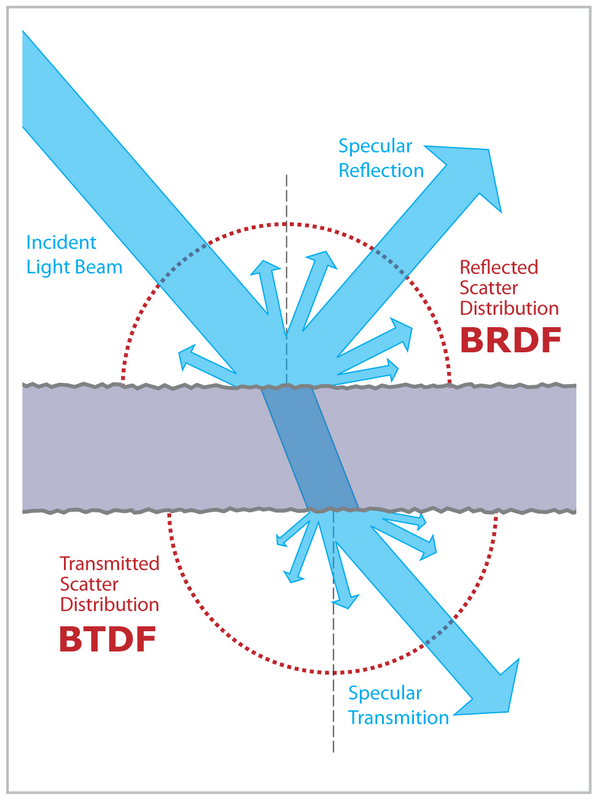
\includegraphics[width=.35\textwidth]{./figs/transmitted.png}
  \caption{透明物体采样示意图}
  \label{fig:transmitted}
\end{figure}

\subsection{随机函数}
如前所叙,算法中主要采用了两种采样概率分布:Cosine Weighted Distribution和Cosine Power Weighted Distribution。

\subsubsection{Cosine Weighted Distribution}
对于Cosine Weighted Distribution,采用如下随机数生成函数:
\begin{equation}
  \begin{split}
    \phi &= 2\pi U_1,  \\
    \theta &= arcsin\big(\sqrt{U_2}\big), \\
    U_1 &\sim Uniform(0, 1),  \\
    U_2 &\sim Uniform(0, 1).
  \end{split}
\end{equation}

\subsubsection{Cosine Power Weighted Distribution}
对于Cosine Power Weighted Distribution,首先我们可以证明其$p(\theta, \phi)$在$\theta \in [0, \frac{\pi}{2}]$且$\phi \in [0, 2\pi]$上的概率累积为$1$:
\begin{equation}
  \begin{split}
    P\big(\frac{\pi}{2}, 2\pi\big)
      &= \int_0^{2\pi} \int_0^{\frac{\pi}{2}}
         \frac{(n_s+1) sin\theta cos^{n_s}\theta}{2\pi}
         d\theta d\phi  \\
      &= -\frac{1}{2\pi} \cdot (2\pi) \cdot \int_0^{\frac{\pi}{2}} d(cos^{n_s+1}\theta)  \\
      &= 1.
  \end{split}
\end{equation}
故可以采用如下随机数生成函数:
\begin{equation}
  \begin{split}
    \phi &= 2\pi U_1,  \\
    \theta &= arccos\big(\sqrt[n_s+1]{U_2}\big),  \\
    U_1 &\sim Uniform(0, 1),  \\
    U_2 &\sim Uniform(0, 1).
  \end{split}
\end{equation}

\subsection{Monte Carlo路径积分}
生成好路径后,对应的Monte Carlo路径积分的计算就十分简单了。 对于每个像素点对应的路径,从路径的终点(光源)出发,逐子路径根据Blinn-Phong或Lambert公式计算亮度的传播,并沿途累乘所有的PDF。回到路径的起点后,求出最终亮度值和累积PDF的商,作为这个像素点的estimator。所有像素点计算完毕后,一轮采样完成。继续对所有像素点进行采样,达到预设的最大采样次数$N_{max}$后再求各次采样的平均,输出最后的渲染结果:
\begin{equation}
  I_e(u, v) = \frac{1}{N_{max}} \sum_{n=1}^{N_{max}} I_e^{(n)}(u, v).
\end{equation}

\subsection{OpenMP并行加速}
整个采样过程具有高度的可并行性——各次采样、各个像素点的采样之间完全没有关联,因此非常适合使用并行加速来提高采样效率。采用CPU上比较方便使用的并行技术OpenMP是一个比较方便的选择。

\newpage
\section{结果展示}
如图~\ref{fig:scene01}和图~\ref{fig:scene02}分别展示了场景1和场景2的运行结果。

\begin{figure}[htbp]
  \centering
  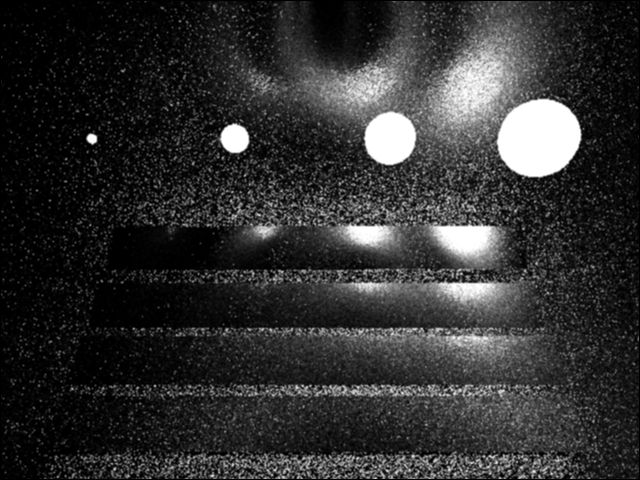
\includegraphics[width=.38\textwidth]{./figs/scene02_0100.png}
  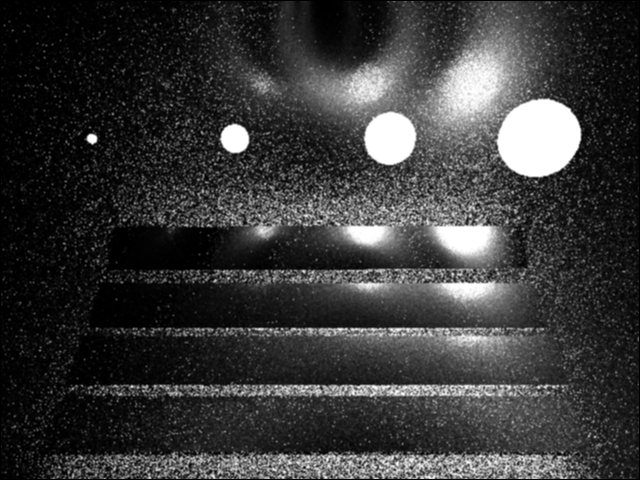
\includegraphics[width=.38\textwidth]{./figs/scene02_0300.png}
  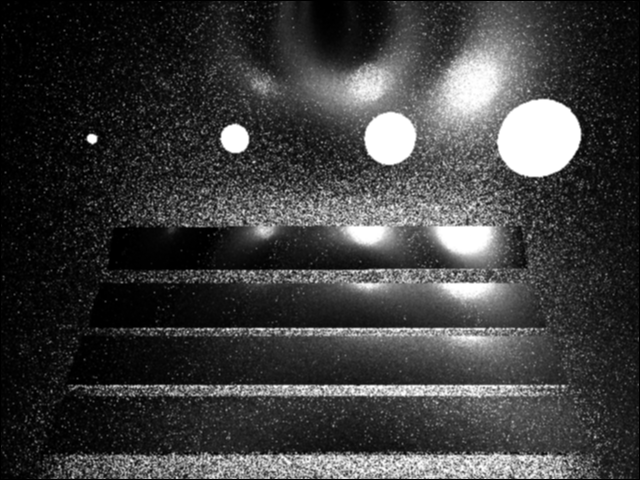
\includegraphics[width=.38\textwidth]{./figs/scene02_0600.png}
  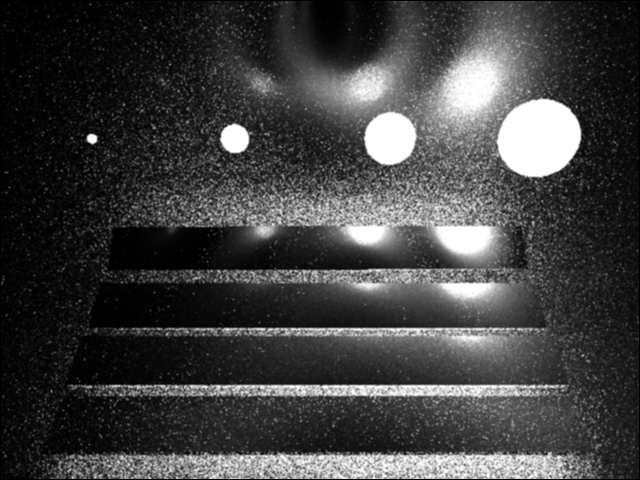
\includegraphics[width=.38\textwidth]{./figs/scene02_1000.png}
  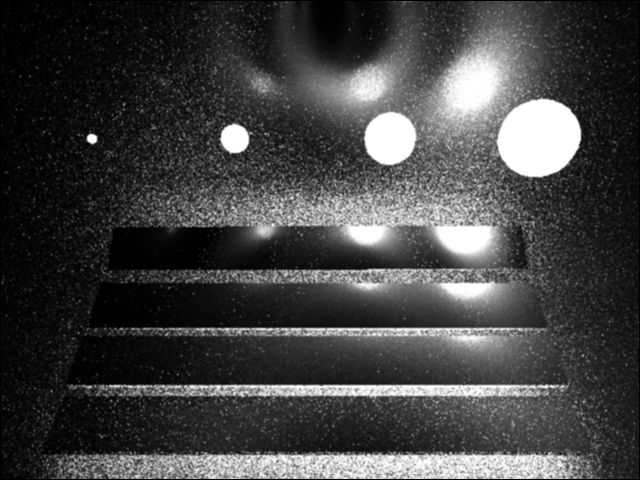
\includegraphics[width=.38\textwidth]{./figs/scene02_1500.png}
  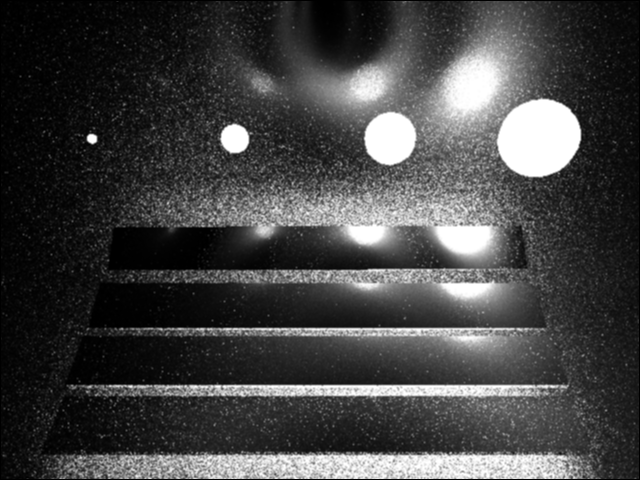
\includegraphics[width=.38\textwidth]{./figs/scene02_2000.png}
  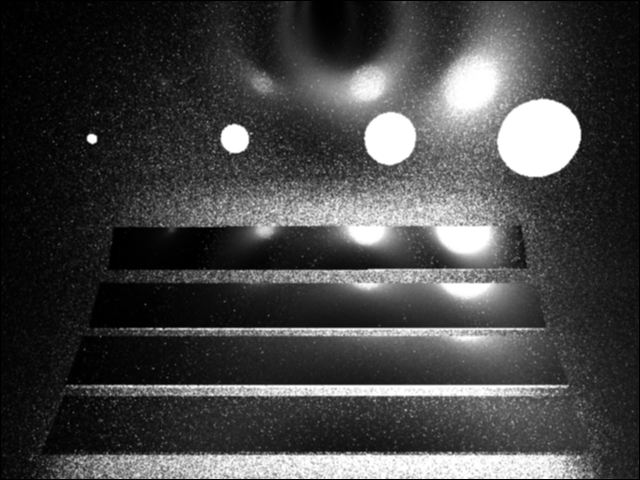
\includegraphics[width=.38\textwidth]{./figs/scene02_4000.png}
  \caption{从左到右、从上到 分别是场景2采样100、300、600、1000、1500、2000、4000次的渲染结果。}
  \label{fig:scene02}
\end{figure}

\begin{figure}[htbp]
  \centering
  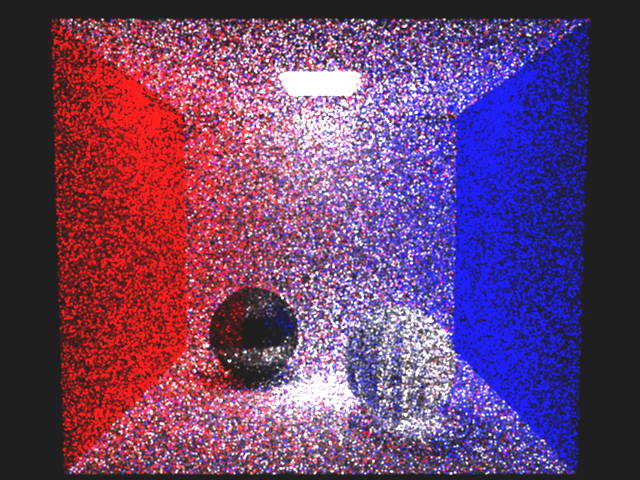
\includegraphics[width=.4\textwidth]{./figs/scene01_00100.png}
  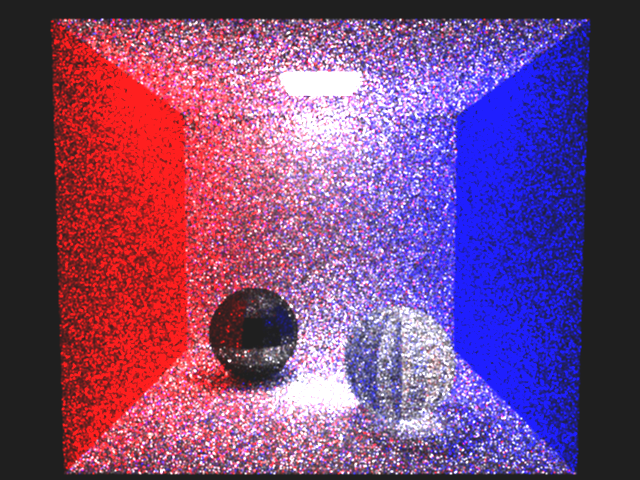
\includegraphics[width=.4\textwidth]{./figs/scene01_00300.png}
  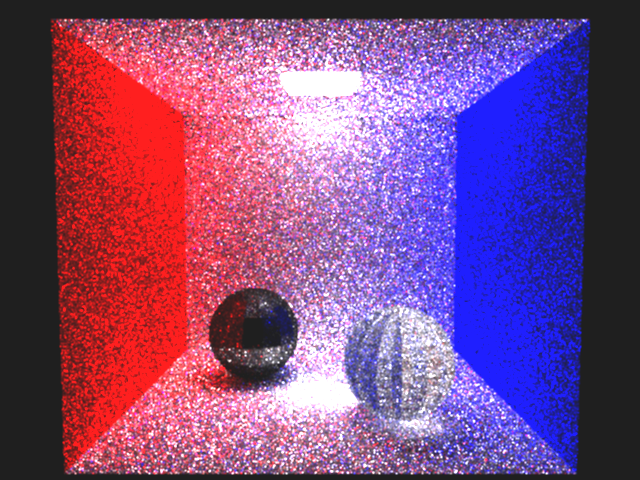
\includegraphics[width=.4\textwidth]{./figs/scene01_00600.png}
  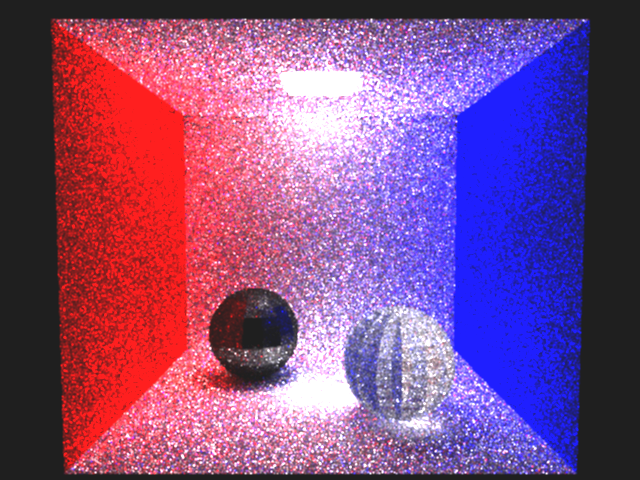
\includegraphics[width=.4\textwidth]{./figs/scene01_01000.png}
  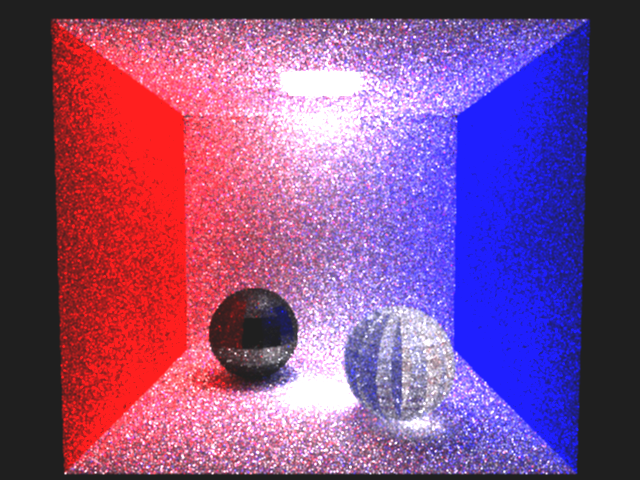
\includegraphics[width=.4\textwidth]{./figs/scene01_01500.png}
  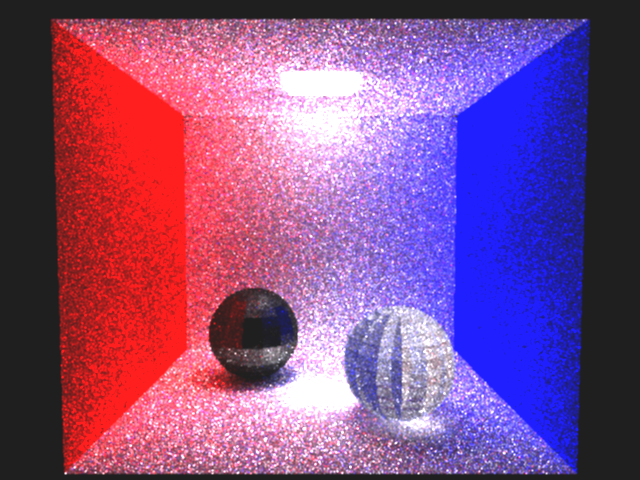
\includegraphics[width=.4\textwidth]{./figs/scene01_02000.png}
  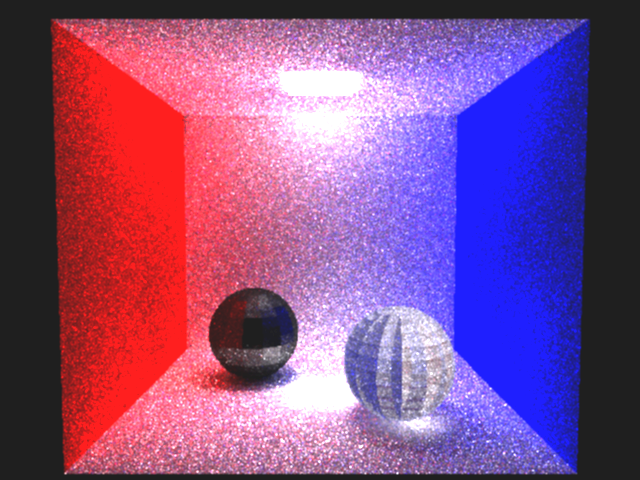
\includegraphics[width=.4\textwidth]{./figs/scene01_04000.png}
  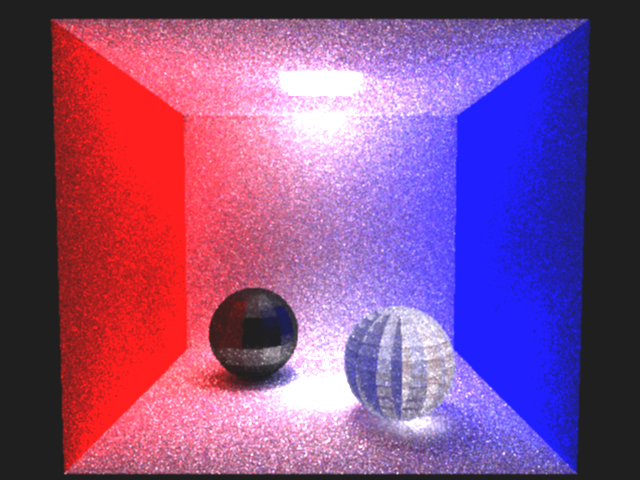
\includegraphics[width=.4\textwidth]{./figs/scene01_06000.png}
  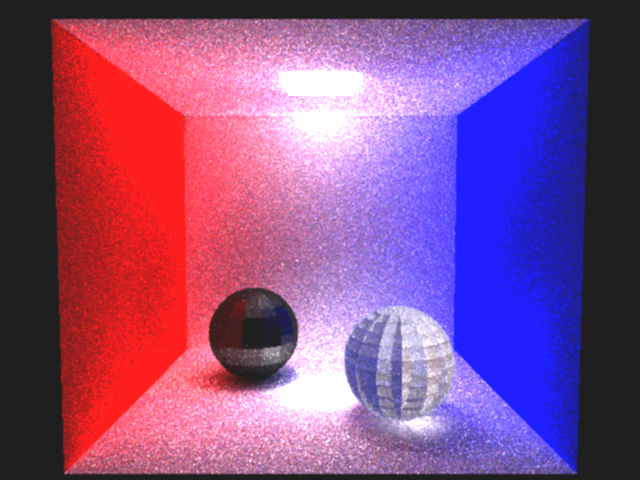
\includegraphics[width=.4\textwidth]{./figs/scene01_10000.png}
  \caption{从左到右、从上到下分别是场景1采样100、300、600、1000、1500、2000、4000、6000、10000次的渲染结果。}
  \label{fig:scene01}
\end{figure}

\newpage
\section{代码说明}
\begin{itemize}\small
  \item 编写语言:C++
  \item 编程环境:Arch Linux,x86\_64 Linux 4.11.3-1-ARCH,GCC 7.1.1
  \item 运行依赖:CMake、Make、支持C++ 11和OpenMP的编译器
\end{itemize}

\subsection{编译运行}
运行以下命令构建程序:
\begin{lstlisting}
mkdir build
cd build
cmake .. -DCMAKE_BUILD_TYPE=Release
make -j$(nproc)
\end{lstlisting}

运行以下命令启动程序:
\begin{lstlisting}
./MonteCarloPathTracing /path/to/.obj depth samples[ samples[ ...]]
\end{lstlisting}

其中\lstinline!depth!指的是最大的路径长度,\lstinline!samples[ samples[ ...]]!是一系列采样的次数。比如:
\begin{lstlisting}
./MonteCarloPathTracing ../examples/scene01.obj 10 300 500 1000 2000
\end{lstlisting}
会对模型文件\lstinline!../examples/scene01.obj!进行300、500、1000、2000次采样并分别输出文件,最大的路径长度是10。最终的结果会以\lstinline!.ppm!的格式保存到模型文件所在目录下。

\end{document}
